\documentclass{my_template}
\usepackage{enumerate}
\usepackage{graphicx}
\usepackage{amsmath}
\Exercisenum{4}
\fellow{Hu Jie}{518370910057}
\group{19}
\title{Polarization of Light}
\begin{document}
    \maketitle
    \tableofcontents
    \newpage
    \section{Introduction \& Theoretical Background}
    \paragraph{}Light is a kind of electro-magnetic wave formed by time-varying perpendicular magnetic and electric field. General we consider the electric field vector with the maximum magnitude as the light vector, which is always perpendicular to the direction along which light propagates. Thus, light is a kind of transverse wave. In natural light, the direction of the oscillation is in all possible direction (on a plane perpendicular to the direction along which light propagates), and the amplitude of these oscillations are all equal. In other words, the electric field vector's distribution is uniform. Therefore, natural light is also called unpolarized light. If, on the other hand, at any given particular time point, the light oscillation is not uniform, this kind of light is called polarized light. 
    \subsection{Polarization of Light}
    \paragraph{} There are many kinds of polarized light. If the light vector's direction is always the same, it will be a linearly polarized light (Figure \ref{fig:linearly polarized light demo}). The direction of the light vector is referred to as the polarization axis. 
    \begin{figure}[!ht]
        \centering
        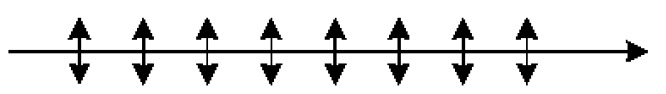
\includegraphics[width=\textwidth]{fig/linearly_polarized_light.png}
        \caption{Linearly polarized light whose polarization axis is parallel to the page plane}
        \label{fig:linearly polarized light demo}
    \end{figure}
    If the end point of the light vector is rotating about the propagation direction of light and its trajectory on a plane is a circle, the light is circularly polarized. If its trajectory is an ellipse, it is called elliptically polarized(Figure \ref{fig:ellipse&circle}).
    \begin{figure}[!ht]
        \centering
        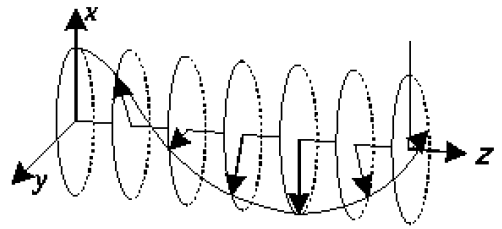
\includegraphics[width=0.5\textwidth]{fig/elliptically_polarized_light.png}
        \caption{Elliptically polarized light}
        \label{fig:ellipse&circle}
    \end{figure}
    If the light is a combination of a polarized light and natural light, it is called partially polarized light.
    \subsection{Polarizer}
    \paragraph{} A polaroid(also known as polarizer) is a device commonly used in labs to generate polarized light. It polarizes the light using the principle of dichroism. It allows the light polarized in a certain direction (direction of the crystal alignment) to pass through the material, while the light polarized in all other directions is absorbed. This turns the incident natural light into linearly polarized. The polaroid can also be used as an analyzer(See the next section).
    \subsection{Malus's Law}
    \paragraph{} Malus's Law is a quantitative law describing the change of the brightness of a linearly polarized light passing through an analyzer. Suppose that we have two polarizers arranged so that their planes are parallel -- the left one plays the role of a polarizer, the other one is an analyzer (Figure \ref{fig:Malus's Law demo}). Let the angle between their transmission directions (polarization axes) be $\theta$. The light is incident normally on the polarizer and then continues to the analyzer. The intensity of the linearly polarized light leaving the analyzer is$$I_{light}=I_{light,0}\cos^2\theta$$
    \begin{figure}[!ht]
        \centering
        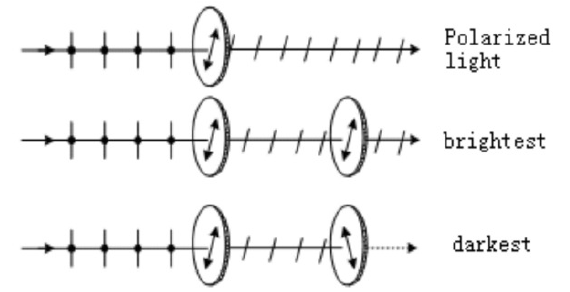
\includegraphics[width=0.7\textwidth]{fig/M_Law_demo.png}
        \caption{Change in the brightness of the light depends on the mutual orientation of the polarizer and the analyzer.}
        \label{fig:Malus's Law demo}
    \end{figure}
    \paragraph{} We can use the analyzer to determine the incident light's polarization. If it is natural light or circularly polarized light, when we rotate the analyzer, the light intensity will remain a constant. If it is partially polarized or elliptically polarized, the minimum intensity will not be zero. If it is linearly polarized, there will be a certain angle where the light intensity becomes zero. 
    \subsection{The Generation of Elliptically and Circularly Polarized Light. Half-wave and Quarter-wave Plates}
    \paragraph{} When a linearly polarized light is incident normally on a crystal plate whose surface is parallel to its optical axis, the light is resolved into two waves: an {\itshape e}-wave with the oscillation direction parallel to the optical axis of the plate (extraordinary axis) and an {\itshape o}-wave whose oscillation direction is perpendicular to the optical axis (ordinary axis)(Figure \ref{fig: e-wave and o-wave}). Suppose the angle between the polarizing axis and the optical axis of the plate is $\alpha$. The two waves propagate in the same direction, but with different speeds. The resulting optical path difference over the thickness $d$ of the plate is $$\Delta=(n_e-n_o)d,$$ where $n_e$ and $n_o$ are the refraction index of the $e$-wave and $o$-wave in the crystal. And the phase difference will be $$\delta=\frac{2\pi(n_e-n_o)d}{\lambda},$$ where $\lambda$ is the wave length of the light.
    \begin{figure}[!ht]
        \centering
        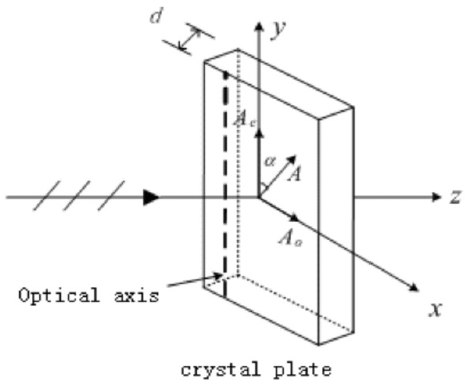
\includegraphics[width=0.5\textwidth]{fig/plate.png}
        \caption{Linearly polarized light passing through a waveplate.}
        \label{fig: e-wave and o-wave}
    \end{figure}
    \paragraph{}As shown in Figure \ref{fig: e-wave and o-wave}, when the light propagates through the crystal plate, the two components of the light vector are 
    \begin{eqnarray*}
        E_x&=&A_o\cos\omega t\\
        E_y&=&A_e\cos(\omega t+\delta),
    \end{eqnarray*}
    where $A_o=A\sin\alpha$, $A_e=A\cos\alpha$. Eliminating time from the above equations one obtains 
    \begin{equation}
        \frac{E_x^2}{A_o^2}+\frac{E_y^2}{A_e^2}-2\frac{E_xE_y}{A_oA_e}\cos\delta=\sin^2\delta.\label{eqn:1}
    \end{equation}
    When the thickness of the plate changes, the optical path difference changes as well. Some cases of particular interest, are discussed below:
    \begin{itemize}
        \item If $\Delta=k\lambda(k=0,1,2,\dots)$, the phase difference $\delta$ will be 0, and Equation \ref{eqn:1} becomes $$E_y=\frac{A_e}{A_o}E_x,$$which is a linear equation. Hence the transmitted light is linearly polarized with the oscillation direction remaining unchanged. A waveplate that satisfies this condition is called a full-wave plate. The light goes through a full-wave plate without changing its polarization state.
        \item If $\Delta=(2k+1)\lambda/2(k=0,1,2,\dots)$, the phase difference $\delta$ will be $\pi$, and Equation \ref{eqn:1} is $$E_y=-\frac{A_e}{A_o}E_x.$$The transmitted light is also linearly polarized with the polarization axis rotated by the angle of 2$\alpha$. A waveplate that satisfies the condition is called 1/2-wave plate or half-wave plate. When a polarized light passes through a half-wave plate, its polarization axis gets rotated by an angle 2$\alpha$. If $\alpha$ = $\pi$/4, then the polarization axis of the transmitted light is perpendicular to that of the incident light.
        \item If $\Delta=(2k+1)\lambda/4(k=0,1,2,\dots)$, the phase difference $\delta$ will be $\pm\pi/2$, and Equation \ref{eqn:1} becomes $$\frac{E_x^2}{A_o^2}+\frac{E_y^2}{A_e^2}=1.$$The transmitted light is elliptically polarized. A waveplate that satisfies the above condition is called a 1/4-wave plate or a quarter-waveplate and is an important optical element in many polarization experiments.
    \end{itemize}
    \paragraph{}If $A_e=A_o=A$, then $E^2_x + E^2_y = A^2$, and the transmitted light is circularly polarized. Since the amplitudes of the $o$-wave and the $e$-wave are both functions of $\alpha$, the polarization state after passing through a 1/4-wave plate will vary, depending on the angle: 
    \begin{itemize}
        \item if $\alpha = 0$, the transmitted light is linearly polarized with the polarization axis parallel to the optical axis of the 1/4-wave plate;
        \item if $\alpha=\pi/2$, the transmitted light is linearly polarized with the polarization axis perpendicular to the optical axis of the 1/4-wave plate;
        \item if $\alpha=\pi/4$, the transmitted light is circularly polarized;
        \item otherwise, the transmitted light is elliptically polarized.
    \end{itemize}
    \section{Apparatus \& Measurement Procedure}
    \subsection{Apparatus}
    The measurement setup consists of: a semiconductor laser, a silicon photo-cell, a UT51 digital universal meter, as well as two polarizers, 1/2-wave and 1/4-wave plates. The elements are placed on an optical bench. The uncertainty of the apparatus is listed in Table \ref{tab:uncertainty}.
    \begin{table}[!ht]
        \centering
        \begin{tabular}{|c|c|}
            \hline
            Apparatus&Uncertainty\\\hline
            Digital Universal Meter&0.001[$\mu$A]\\\hline
            Two polarizers, 1/2-wave and 1/4-wave plates&2[$^\circ$]\\\hline
        \end{tabular}
        \caption{The uncertainty of the apparatus used in this lab section}
        \label{tab:uncertainty}
    \end{table}
    \subsection{Measurement Procedure}
    \subsubsection{Demostration of Malus's Law}
    \begin{enumerate}
        \item Take the polarizers and the plates off the optical bench. Turn on the universal meter and the laser. Make sure that laser is incident into the transmitter with the mark ``$\Phi 6$''. After we have got some readings on the universal meter, do not adjust the laser's direction for the rest of the lab.
        \item Put one of the polarizers on the optical bench. Adjust the direction so that the reflection light is not too deviated from the source. Make sure that the reading on the universal meter is around 0.8 -- 1 [$\mu$A].
        \item Put the other polarizer on the optical bench. Rotate it so that the reading becomes zero on the universal meter. Let this angle be 90$^\circ$.
        \item Rotate the analyzer for 5$^\circ$(the direction does not matter), and record the reading. Repeat this until the rotation angle becomes 0$^\circ$.
    \end{enumerate}
    \subsubsection{Linearly Polarized Light and the Half-wave Plate}
    \begin{enumerate}
        \item Put the half wave plate on the optical bench between the polarizer and the analyzer.
        \item Rotate the analyzer until the reading becomes zero on the universal meter. Record the angle on the analyzer.\label{enum:2}
        \item Rotate the half-wave plate for 10$^\circ$, and then rotate the analyzer until the reading on the universal meter becomes zero again. Read the angle on the analyzer and record the difference of it between the angle in Step \ref{enum:2}. \label{enum:3}
        \item  Repeat Step \ref{enum:3} until the half-wave plate has rotated 90$^\circ$.
    \end{enumerate}
    \subsubsection{Circularly and Elliptically Polarized Light and the 1/4-wave Plate}
    \begin{enumerate}
        \item Take the half wave plate off, and then rotate the analyzer until the reading becomes zero.
        \item Put on the quarter-wave plate, and the rotate the plate until the reading becomes zero again. Record the angle both on the analyzer and the plate.\label{enum:2.2}
        \item Take this reading as the data for $\theta=90^\circ$. Rotate the analyzer for 10$^\circ$, record it as the next data.\label{enum:2.3}
        \item Repeat Step \ref{enum:2.3} until the analyzer is rotated for a full round.
        \item Choose the maximum value of current in the 36 results and make it the ``Maximum Electric Current $I_0$''.\label{enum:2.5}
        \item Rotate the analyzer to its angle in Step \ref{enum:2.2}, and then rotate the quarter plate for 20$^\circ$. Repeat Step \ref{enum:2.3} to \ref{enum:2.5}.
        \item Rotate the quarter plate for another 25$^\circ$, and repeat step \ref{enum:2.3} to \ref{enum:2.5}.
    \end{enumerate}
    \section{Result}
    \subsection{Demostration of Malus's Law}\label{sec:malus}
    \begin{table}[!ht]
        \centering
        \begin{tabular}{|c|c||c|c|}
            \hline
            \multicolumn{2}{|c||}{Maximum Electric Current $I_0$}&\multicolumn{2}{c|}{$0.780\pm 0.001[\mu$A]}\\\hline
            $\theta[^\circ]\pm 2[^\circ]$&$I[\mu{\rm A}]\pm 0.001[\mu$A]&$\theta[^\circ]\pm 2[^\circ]$&$I[\mu{\rm A}]\pm 0.001[\mu$A]\\\hline
            0&0.780&50&0.334\\\hline
            5&0.779&55&0.259\\\hline
            10&0.766&60&0.207\\\hline
            15&0.742&65&0.148\\\hline
            20&0.702&70&0.094\\\hline
            25&0.659&75&0.056\\\hline
            30&0.607&80&0.028\\\hline
            35&0.538&85&0.008\\\hline
            40&0.467&90&0.000\\\hline
            45&0.404&&\\\hline
        \end{tabular}
        \caption{Measurement data of Malus's law demostration}
        \label{tab:Malus's Law}
    \end{table}
    \paragraph{} Table \ref{tab:Malus's Law} is the result of the verification of Malus's law. I performed a linear fit of the $I_0/I$ versus $\cos^2\theta$ using the data in Table \ref{tab:Malus's Law Linear Fit}. When $I=0.780[\mu$A] and $\theta=0^\circ$, the sample calculations are as follows: 
    \begin{eqnarray*}
        \frac{I}{I_0}=\frac{0.780}{0.780}=1.0000\pm 0.0018\\
        \cos^2\theta=\cos^2(0\times\pi/180)=1\pm 0.
    \end{eqnarray*}
    \begin{table}[!ht]
        \centering
        \begin{tabular}{|c|c||c|c|}
            \hline
            $I/I_0$&Uncertainty&$\cos^2\theta$&Uncertainty\\\hline
            1.0000&0.0018&1&0\\\hline
            0.9987&0.0018&0.992&0.006\\\hline
            0.9821&0.0018&0.970&0.012\\\hline
            0.9513&0.0018&0.93&0.02\\\hline
            0.9000&0.0017&0.88&0.03\\\hline
            0.8449&0.0017&0.82&0.03\\\hline
            0.7782&0.0016&0.75&0.03\\\hline
            0.6897&0.0016&0.67&0.03\\\hline
            0.5987&0.0015&0.59&0.03\\\hline
            0.5179&0.0014&0.50&0.03\\\hline
            0.4282&0.0014&0.41&0.03\\\hline
            0.3321&0.0014&0.33&0.03\\\hline
            0.2654&0.0013&0.25&0.03\\\hline
            0.1897&0.0013&0.18&0.03\\\hline
            0.1205&0.0013&0.12&0.02\\\hline
            0.0718&0.0013&0.067&0.018\\\hline
            0.0359&0.0013&0.030&0.012\\\hline
            0.0103&0.0013&0.007&0.006\\\hline
            0.0000&0.0013&0&0\\\hline
        \end{tabular}
        \caption{Data for linear fit of Malus's law demostration}
        \label{tab:Malus's Law Linear Fit}
    \end{table}
    Figure \ref{fig: Malus's Law linear fit} is the graph of the linear fit. From it we can directly read that $$\frac{I}{I_0\cos^2\theta}=1.01\pm 0.01.$$ As the expected result($I/I_0\cos^2\theta=1$) is within the uncertainty, we can conclude that Malus's Law has been verified.
    \begin{figure}[!ht]
        \centering
        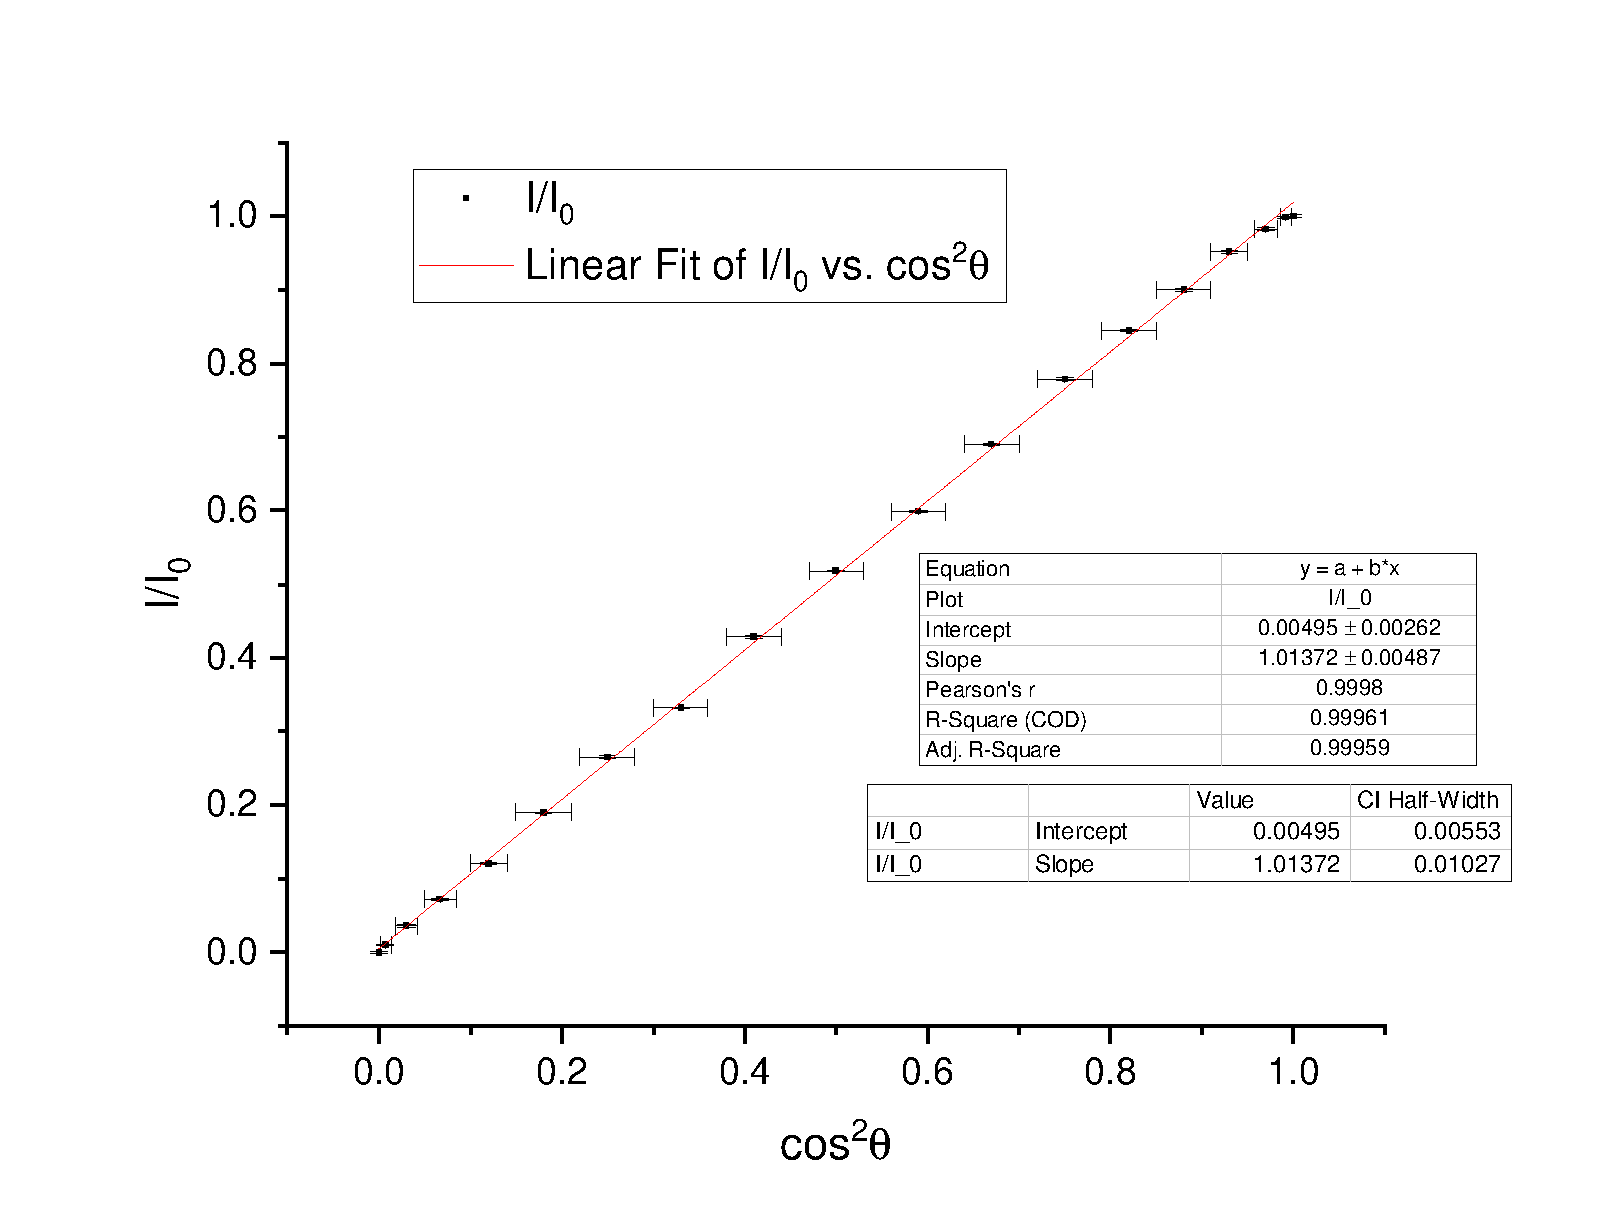
\includegraphics[width=0.7\textwidth]{fig/malus_law.pdf}
        \caption{The linear fit of Malus's law demostration}
        \label{fig: Malus's Law linear fit}
    \end{figure}
    \subsection{Linearly Polarized Light and the Half-wave Plate}
    \begin{table}[!ht]
        \centering
        Uncertainty of the angle: $\pm 2[^\circ]$
        \begin{tabular}{|c|c|}
            \hline
            Rotation angle of the 1/2-wave plate[$^\circ$]&Rotation angle of the analyzer[$^\circ$]\\\hline
            initial&0\\\hline
            10&17\\\hline
            20&32\\\hline
            30&58\\\hline
            40&78\\\hline
            50&98\\\hline
            60&118\\\hline
            70&139\\\hline
            80&158\\\hline
            90&178\\\hline
        \end{tabular}
        \caption{Measurement data for the 1/2-wave plate}
        \label{tab:half plate}
    \end{table}
    \paragraph{} Table \ref{tab:half plate} is the result of the linear polarized light passing through a half wave plate. The expected result is that $\Delta\theta=2\theta$, where $\Delta\theta$ is the rotation angle of the analyzer, and $\theta$ is the rotation angle of the half-wave plate. The data used in the linear fit is listed in Table \ref{tab:half linear fit}.
    \begin{table}
        \centering
        \begin{tabular}{|c|c|c|c|}
            \hline
            $\theta$[$^\circ$]&Uncertainty[$^\circ$]&$\Delta\theta$[$^\circ$]&Uncertainty\\\hline
            0&2&0&2\\\hline
            10&2&17&2\\\hline
            20&2&32&2\\\hline
            30&2&58&2\\\hline
            40&2&78&2\\\hline
            50&2&98&2\\\hline
            60&2&118&2\\\hline
            70&2&139&2\\\hline
            80&2&158&2\\\hline
            90&2&178&2\\\hline
        \end{tabular}
        \caption{The data for linear fit of $\Delta\theta$ vs. $\theta$}
        \label{tab:half linear fit}
    \end{table}
    \begin{figure}[!ht]
        \centering
        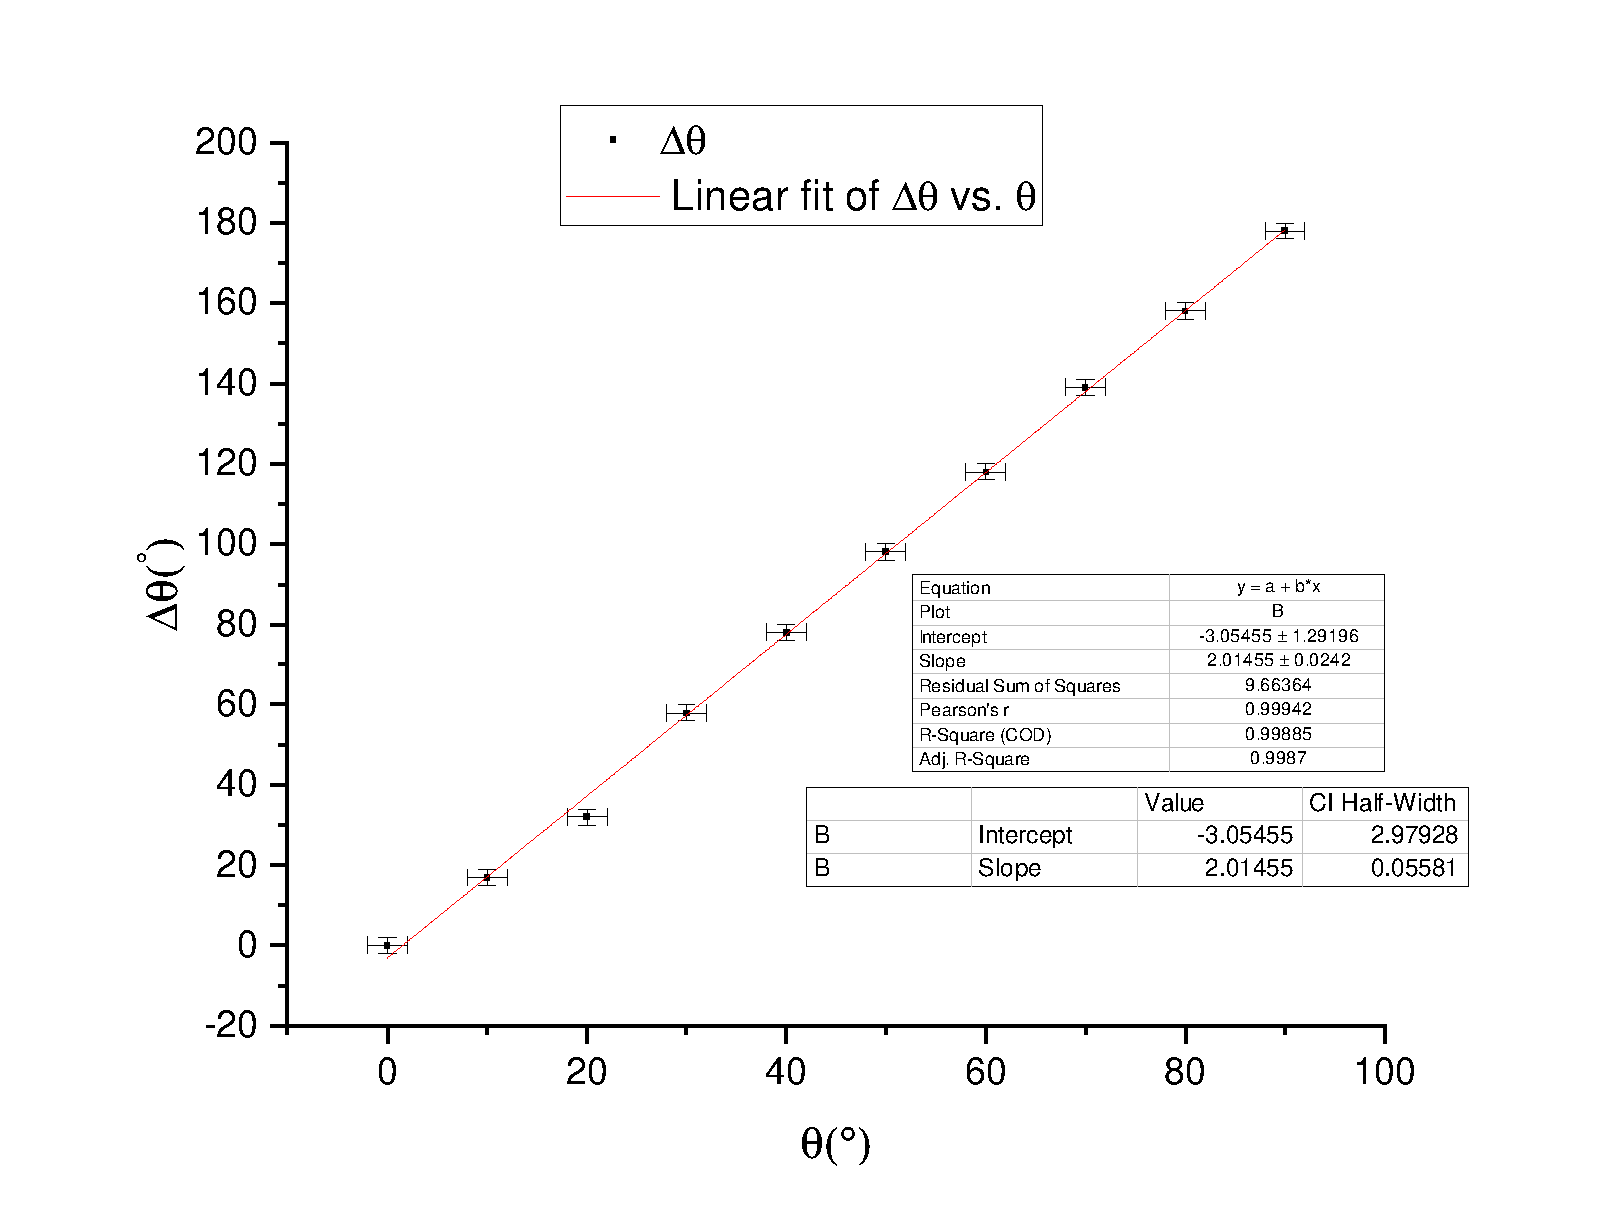
\includegraphics[width=0.7\textwidth]{fig/half.pdf}
        \caption{The linear fit of $\Delta\theta$ vs. $\theta$}
        \label{fig: half linear fit}
    \end{figure}
    From Figure \ref{fig: half linear fit}, we can read that $$\frac{\Delta\theta}{\theta}=2.01\pm 0.06.$$
    \subsection{The light intensity when the quarter wave plate's angle is 0$^\circ$}\label{sec:0}
    \begin{table}[!ht]
        \centering
        \begin{tabular}{|c|c||c|c|}
            \hline
            \multicolumn{4}{|c|}{Rotation angle of 1/4-wave plate: 0$[^\circ]$}\\\hline
            \multicolumn{2}{|c||}{Maximum Electric Current $I_0$}&\multicolumn{2}{c|}{$0.498\pm 0.001[\mu$A]}\\\hline
            $\theta[^\circ]\pm 2[^\circ]$&$I[\mu \rm A]\pm 0.001 [\mu A]$&$\theta[^\circ]\pm 2[^\circ]$&$I[\mu \rm A]\pm 0.001 [\mu A]$\\\hline
            0&0.487&180&0.498\\\hline
            10&0.472&190&0.481\\\hline
            20&0.440&200&0.440\\\hline
            30&0.379&210&0.379\\\hline
            40&0.298&220&0.294\\\hline
            50&0.208&230&0.203\\\hline
            60&0.126&240&0.116\\\hline
            70&0.056&250&0.052\\\hline
            80&0.013&260&0.011\\\hline
            90&0.000&270&0.001\\\hline
            100&0.016&280&0.020\\\hline
            110&0.061&290&0.067\\\hline
            120&0.133&300&0.139\\\hline
            130&0.221&310&0.227\\\hline
            140&0.308&320&0.315\\\hline
            150&0.387&330&0.392\\\hline
            160&0.452&340&0.452\\\hline
            170&0.492&350&0.498\\\hline
        \end{tabular}
        \caption{Measurement data for the 1/4-wave plate(rotation angle 0$^\circ$).}
        \label{tab:0 quarterplate}
    \end{table}
    \paragraph{} Table \ref{tab:0 quarterplate} is the original data for the light intensity of the transmitted light passing through a quarter wave plate. I drew the relation between $\sqrt{I/I_0}$ vs. $\theta$ under polar coordinate using the modified data in Table \ref{tab:plot0} and get Figure \ref{fig:quarter0}.
    \begin{table}[!ht]
        \centering
        \begin{tabular}{|c|c|c|c|}
            \hline
            $\sqrt{\frac{I}{I_0}}$&Uncertainty&$\theta[^\circ]$&Uncertainty[$^\circ$]\\\hline
            0.9889&0.0014&0&2\\\hline
            0.9736&0.0014&10&2\\\hline
            0.9400&0.0014&20&2\\\hline
            0.8723&0.0015&30&2\\\hline
            0.7736&0.0015&40&2\\\hline
            0.6463&0.0017&50&2\\\hline
            0.503&0.002&60&2\\\hline
            0.335&0.002&70&2\\\hline
            0.162&0.006&80&2\\\hline
            0&0$^\star$&90&2\\\hline
            0.179&0.006&100&2\\\hline
            0.350&0.003&110&2\\\hline
            0.517&0.002&120&2\\\hline
            0.6662&0.0017&130&2\\\hline
            0.7864&0.0015&140&2\\\hline
            0.8815&0.0014&150&2\\\hline
            0.9527&0.0014&160&2\\\hline
            0.9940&0.0014&170&2\\\hline
            1.0000&0.0014&180&2\\\hline
            0.9828&0.0014&190&2\\\hline
            0.9400&0.0014&200&2\\\hline
            0.8724&0.0015&210&2\\\hline
            0.7684&0.0015&220&2\\\hline
            0.6385&0.0017&230&2\\\hline
            0.483&0.002&240&2\\\hline
            0.323&0.003&250&2\\\hline
            0.149&0.007&260&2\\\hline
            0.04&0.02&270&2\\\hline
            0.200&0.005&280&2\\\hline
            0.367&0.003&290&2\\\hline
            0.528&0.002&300&2\\\hline
            0.6752&0.0016&310&2\\\hline
            0.7953&0.0015&320&2\\\hline
            0.8872&0.0014&330&2\\\hline
            0.9527&0.0014&340&2\\\hline
            1.0000&0.0014&350&2\\\hline
        \end{tabular}
        \caption{The data for the polar coordinate plot when angle is 0$^\circ$}
        \label{tab:plot0}
        $^\star$Here the uncertainty according to the formula is infinity. This is due to the fact that there is zero on the denominator. I consider it zero because this data is the base of the experiment. I delibrately set it to be zero.
    \end{table}
    \begin{figure}[!ht]
        \centering
        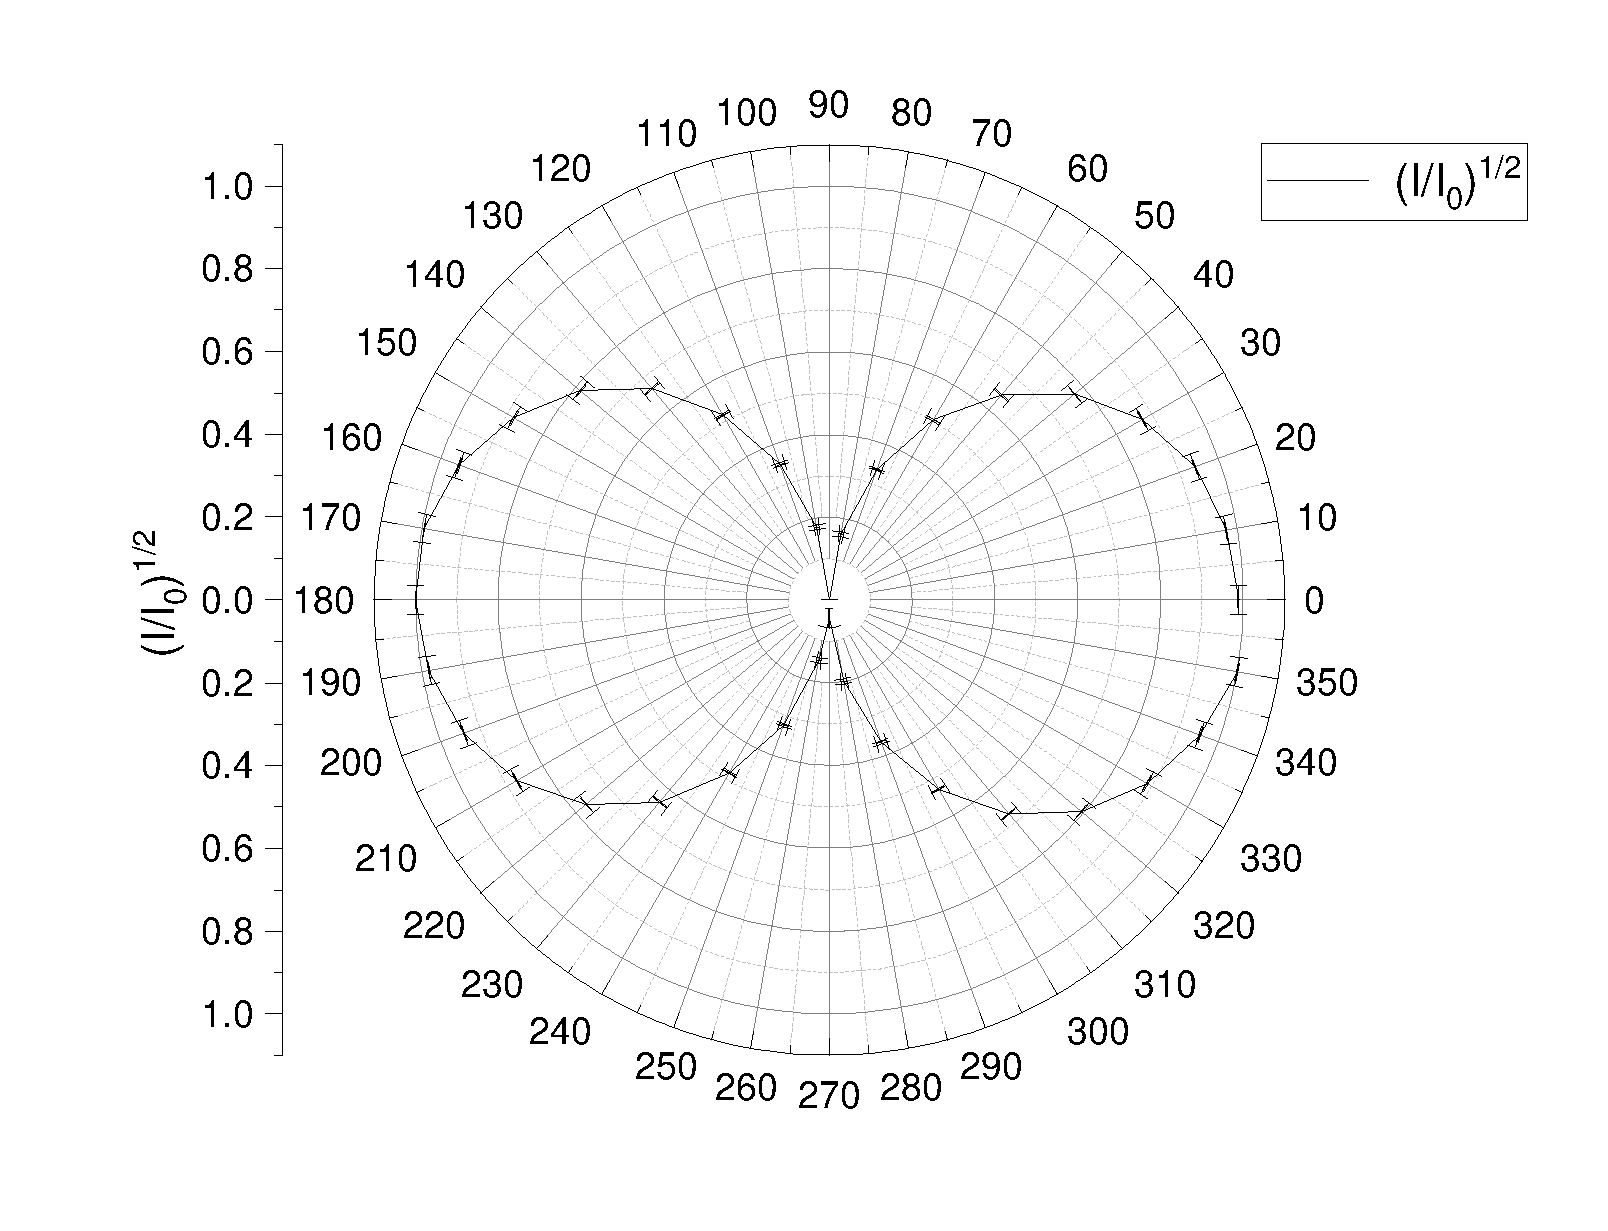
\includegraphics[width=\textwidth]{fig/quarter0.pdf}
        \caption{The graph of $\sqrt{I/I_0}$ vs. $\theta$ in polar coordinate when angle is 0$^\circ$}
        \label{fig:quarter0}
    \end{figure}
    \subsection{The light intensity when the angle is 20$^\circ$}\label{sec:20}
    \paragraph{} Table \ref{tab:20 quarterplate} is the original data in this section. I tried to plot the relation of $\sqrt{I/I_0}$ vs. $\theta$ in polar coordinate with data in Table \ref{tab:plot20}, and got Figure \ref{fig:quarter20}. Note that there is a point outside the trajectory. That point is the point when the rotation angle is 70$^\circ$.
    \begin{table}[!ht]
        \centering
        \begin{tabular}{|c|c||c|c|}
            \hline
            \multicolumn{4}{|c|}{Rotation angle of 1/4-wave plate: 20$[^\circ]$}\\\hline
            \multicolumn{2}{|c||}{Maximum Electric Current $I_0$}&\multicolumn{2}{c|}{$0.446\pm 0.001[\mu$A]}\\\hline
            $\theta[^\circ]\pm 2[^\circ]$&$I[\mu \rm A]\pm 0.001 [\mu A]$&$\theta[^\circ]\pm 2[^\circ]$&$I[\mu \rm A]\pm 0.001 [\mu A]$\\\hline
            0&0.387&180&0.382\\\hline
            10&0.337&190&0.320\\\hline
            20&0.277&200&0.265\\\hline
            30&0.213&210&0.208\\\hline
            40&0.154&220&0.151\\\hline
            50&0.112&230&0.107\\\hline
            60&0.083&240&0.081\\\hline
            70&0.077&250&0.074\\\hline
            80&0.097&260&0.088\\\hline
            90&0.128&270&0.127\\\hline
            100&0.189&280&0.180\\\hline
            110&0.248&290&0.237\\\hline
            120&0.304&300&0.301\\\hline
            130&0.352&310&0.371\\\hline
            140&0.410&320&0.420\\\hline
            150&0.438&330&0.430\\\hline
            160&0.445&340&0.446\\\hline
            170&0.416&350&0.425\\\hline
        \end{tabular}
        \begin{tabular}{|c|c|}
            \hline
            \multicolumn{2}{|c|}{Rotation angle of the quarter wave plate: 70$^\circ$}\\\hline
            $\theta[^\circ]\pm 2[^\circ]$&23\\\hline
            $I[\mu \rm A]\pm 0.001[\mu A]$&0.481\\\hline
        \end{tabular}
        \caption{Measurement data for the 1/4-wave plate(rotation angle 20$^\circ$ and 70$^\circ$).}
        \label{tab:20 quarterplate}
    \end{table}
    \begin{table}[!ht]
        \centering
        \begin{tabular}{|c|c|c|c|}
            \hline
            $\sqrt{\frac{I}{I_0}}$&Uncertainty&$\theta[^\circ]$&Uncertainty[$^\circ$]\\\hline
            0.9315&0.0016&0&2\\\hline
            0.8693&0.0016&10&2\\\hline
            0.7881&0.0017&20&2\\\hline
            0.6911&0.0018&30&2\\\hline
            0.588&0.002&40&2\\\hline
            0.501&0.002&50&2\\\hline
            0.431&0.003&60&2\\\hline
            0.416&0.003&70&2\\\hline
            0.466&0.002&80&2\\\hline
            0.536&0.002&90&2\\\hline
            0.6510&0.0019&100&2\\\hline
            0.7457&0.0017&110&2\\\hline
            0.8256&0.0016&120&2\\\hline
            0.8884&0.0016&130&2\\\hline
            0.9588&0.0016&140&2\\\hline
            0.9910&0.0016&150&2\\\hline
            0.9989&0.0016&160&2\\\hline
            0.9658&0.0016&170&2\\\hline
            0.9255&0.0016&180&2\\\hline
            0.8470&0.0016&190&2\\\hline
            0.778&0.0017&200&2\\\hline
            0.6829&0.0018&210&2\\\hline
            0.582&0.002&220&2\\\hline
            0.490&0.002&230&2\\\hline
            0.426&0.003&240&2\\\hline
            0.407&0.003&250&2\\\hline
            0.444&0.003&260&2\\\hline
            0.534&0.002&270&2\\\hline
            0.6353&0.0019&280&2\\\hline
            0.7290&0.0017&290&2\\\hline
            0.8215&0.0017&300&2\\\hline
            0.9121&0.0016&310&2\\\hline
            0.9704&0.0016&320&2\\\hline
            0.9819&0.0016&330&2\\\hline
            1.0000&0.0016&340&2\\\hline
            0.9762&0.0016&350&2\\\hline
        \end{tabular}
        \caption{The data for the polar coordinate plot when angle is 20$^\circ$}
        \label{tab:plot20}
    \end{table}
    \begin{figure}[!ht]
        \centering
        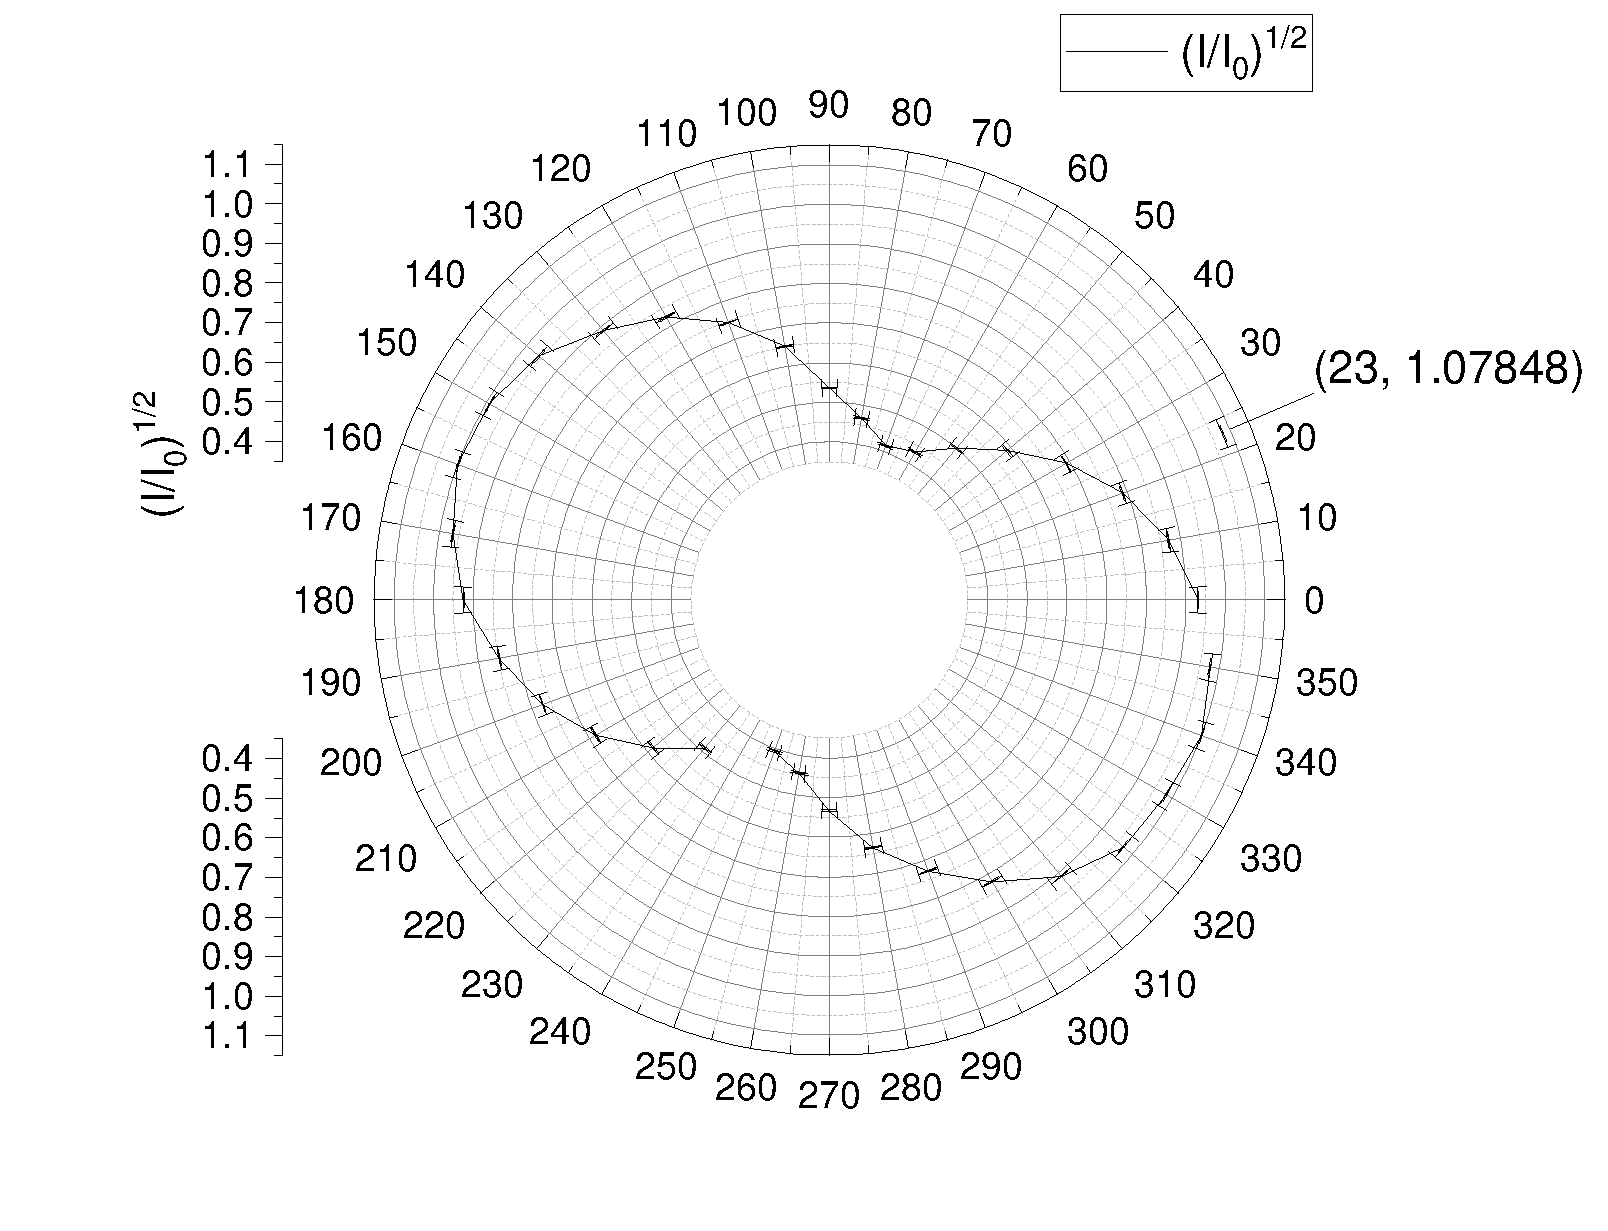
\includegraphics[width=\textwidth]{fig/quarter20.pdf}
        \caption{The graph of $\sqrt{I/I_0}$ vs. $\theta$ in polar coordinate when rotation angle is 20$^\circ$}
        \label{fig:quarter20}
    \end{figure}
    \subsection{The angle of the quarter wave plate is 45$^\circ$}\label{sec:45}
    \paragraph{} Table \ref{tab:45 quarterplate} is the original data for this part. I tried to apply a linear fit with the data and get a graph of $\sqrt{I/I_0}$ vs. $\theta$. Table \ref{tab:linearfitof45} is the data I used to perform the fit and I got Figure \ref{fig:linearfit45}.
    \begin{table}[!ht]
        \centering
        \begin{tabular}{|c|c||c|c|}
            \hline
            \multicolumn{4}{|c|}{Rotation angle of 1/4-wave plate: 45$[^\circ]$}\\\hline
            \multicolumn{2}{|c||}{Maximum Electric Current $I_0$}&\multicolumn{2}{c|}{$0.291\pm 0.001[\mu$A]}\\\hline
            $\theta[^\circ]\pm 2[^\circ]$&$I[\mu \rm A]\pm 0.001 [\mu A]$&$\theta[^\circ]\pm 2[^\circ]$&$I[\mu \rm A]\pm 0.001 [\mu A]$\\\hline
            0&0.224&180&0.220\\\hline
            10&0.236&190&0.227\\\hline
            20&0.248&200&0.235\\\hline
            30&0.263&210&0.249\\\hline
            40&0.274&220&0.260\\\hline
            50&0.285&230&0.275\\\hline
            60&0.291&240&0.278\\\hline
            70&0.285&250&0.278\\\hline
            80&0.282&260&0.275\\\hline
            90&0.278&270&0.269\\\hline
            100&0.274&280&0.260\\\hline
            110&0.258&290&0.247\\\hline
            120&0.244&300&0.238\\\hline
            130&0.230&310&0.232\\\hline
            140&0.222&320&0.225\\\hline
            150&0.214&330&0.221\\\hline
            160&0.215&340&0.219\\\hline
            170&0.217&350&0.215\\\hline
        \end{tabular}
        \caption{Measurement data for the 1/4-wave plate(rotation angle 45$^\circ$).}
        \label{tab:45 quarterplate}
    \end{table}
    \begin{table}[!ht]
        \centering
        \begin{tabular}{|c|c|c|c|}
            \hline
            $\sqrt{\frac{I}{I_0}}$&Uncertainty&$\theta[^\circ]$&Uncertainty[$^\circ$]\\\hline
            0.877&0.002&0&2\\\hline
            0.901&0.002&10&2\\\hline
            0.923&0.002&20&2\\\hline
            0.951&0.002&30&2\\\hline
            0.970&0.002&40&2\\\hline
            0.990&0.002&50&2\\\hline
            1.000&0.002&60&2\\\hline
            0.990&0.002&70&2\\\hline
            0.984&0.002&80&2\\\hline
            0.977&0.002&90&2\\\hline
            0.970&0.002&100&2\\\hline
            0.942&0.002&110&2\\\hline
            0.916&0.002&120&2\\\hline
            0.889&0.002&130&2\\\hline
            0.873&0.002&140&2\\\hline
            0.858&0.002&150&2\\\hline
            0.860&0.002&160&2\\\hline
            0.864&0.002&170&2\\\hline
            0.869&0.002&180&2\\\hline
            0.883&0.002&190&2\\\hline
            0.899&0.002&200&2\\\hline
            0.925&0.002&210&2\\\hline
            0.945&0.002&220&2\\\hline
            0.972&0.002&230&2\\\hline
            0.977&0.002&240&2\\\hline
            0.977&0.002&250&2\\\hline
            0.972&0.002&260&2\\\hline
            0.961&0.002&270&2\\\hline
            0.945&0.002&280&2\\\hline
            0.921&0.002&290&2\\\hline
            0.904&0.002&300&2\\\hline
            0.893&0.002&310&2\\\hline
            0.879&0.002&320&2\\\hline
            0.871&0.002&330&2\\\hline
            0.868&0.002&340&2\\\hline
            0.860&0.002&350&2\\\hline
        \end{tabular}
        \caption{The data for linear fit in Section \ref{sec:45}}
        \label{tab:linearfitof45}
    \end{table}
    \begin{figure}[!ht]
        \centering
        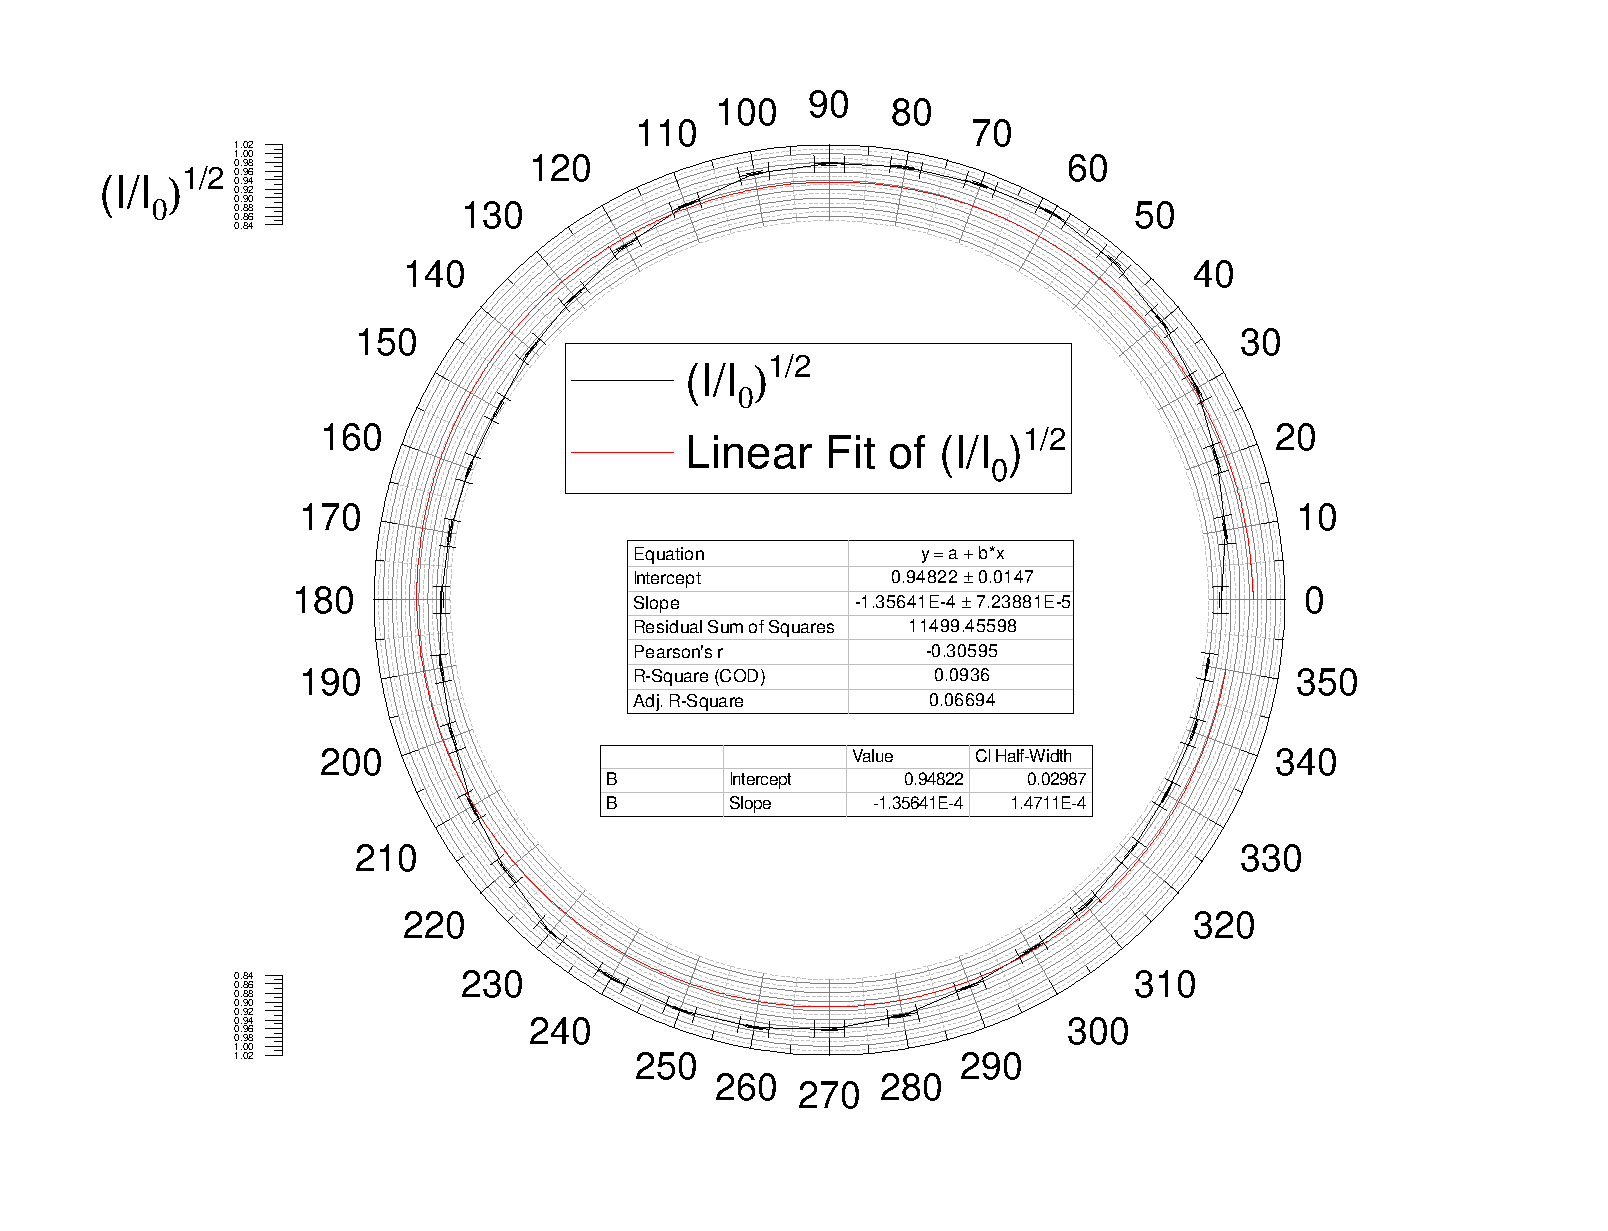
\includegraphics[width=\textwidth]{fig/Linearfitfor45.pdf}
        \caption{The linear fit of $\sqrt{\frac{I}{I_0}}$ vs. $\theta$}
        \label{fig:linearfit45}
    \end{figure}
    In Figure \ref{fig:linearfit45}, we can read the slope(the ratio of $\sqrt{\frac{I}{I_0}}$ and $\theta$) is $-0.00014\pm 0.00007$. This is quite close to zero. However, as the Pearson's r and R-Square here is not close to 1, the linear fit does not work quite well. 
    \section{Discussion}
    \subsection{The demonstration of Malus's law}
    \paragraph{} The verification of Malus's law is quite successful. From Figure \ref{fig: Malus's Law linear fit}, we can conclude that $$\frac{I}{I_0\cos^2\theta}=1.01\pm 0.01.$$ The expected value of this ration is 1, which is within the range of the confidence interval. The uncertainty mainly comes from the error of the universal meter, as I suppose based on this result. Therefore, the intensity of the transmitted light is directly proportional to the incident light intensity and the square of the cosine of the angle of the transmission direction of the polarizer and the analyzer. i.e., $$I_{0,light}=I_0\cos^2\theta$$
    \subsection{Linearly Polarized Light and Half Wave Plate}
    \paragraph{} When I rotate the half wave plate for a full round, the light intensity will vanish twice. Also, if I rotate the analyzer, it will also vanish twice. This is because the transmission light is linearly polarized. The light intensity will vanish when the light vector is orthogonal to the direction of transmission allowed by the analyzer, and it has two direction in a full round. The transmission light after a linearly polarized light is incident to a half wave plate will have a light vector rotated 2$\alpha$, where $\alpha$ is the angle between the polarizing axis and the optical axis of the plate.
    \vspace{-5mm}
    \paragraph{}The result of the linear fit tells us that $$\frac{\Delta\theta}{\theta}=2.01\pm 0.06.$$ The expected ratio is $2$, which is in the confidence interval. So the experiment is quite successful. The uncertainty mainly came from the error of the experiment apparatus, including the universal meter and the protractor on the analyzer and the plate.
    \subsection{Linearly Polarized Light through Quarter-wave Plate when angle is 0$^\circ$ }
    \paragraph{} In this section, we let a linearly polarized light incident onto a quarter wave plate with angle 0$^\circ$. From Figure \ref{fig:quarter0}, we can see that there are two angles where the intensity goes to zero. This means that the transmission light is also a linearly polarized light. However, as we did not rotate the quarter wave plate, we cannot find out the change of the direction of the light vector of the incident light. 
    \subsection{Linearly Polarized Light through Quarter-wave Plate when angle is 20$^\circ$}
    \paragraph{} When the quarter wave plate is rotated for 20$^\circ$, the transmission light becomes elliptically polarized. When I rotate the analyzer for a full round, there is no point where the intensity vanishes. In Figure \ref{fig:quarter20}, I have included an extra point, which is marked with its coordinate. This point is a datum where the rotation angle of the quarter wave plate is 70$^\circ$ and the analyzer at a random angle $\theta$. It should be on the trajectory of the graph. However, as we can see, it is not. A possible explanation for this is that the quarter wave plate we used in lab is not symmetric as it should be. Or it may be the outside light like the torch that interfered the single measurement when rotation angle is $\theta$. 
    \subsection{Linearly Polarized Light through Quarter-wave Plate when angle is 45$^\circ$}
    \paragraph{}When the quarter wave plate is rotated for 45$^\circ$, the transmission light should be circularly polarized, which means that when we rotate the analyzer, the intensity of the transmission light should not change. However, this is not the case. I applied linear fit in Figure \ref{fig:linearfit45}. Although the slope it gives is $$\frac{\sqrt{\frac{I}{I_0}}}{\theta}=0.00014\pm 0.00007,$$ which is quite close to zero, as we have expected, the Pearson's r for this linear fit is -0.306, which makes the linear fit not so valid. The reasons may include the following:
    \begin{enumerate}
        \item The quarter wave plate is not ideal. In some direction the light is blocked because of the plate's inner structure.
        \item The thickness of the plate does not strictly makes the phase difference to be $\pm\frac{\pi}{2}$, probably because of grinding.
        \item We did not set the angle of rotation to be exactly $45^\circ$, there are some uncertainties on the quarter-wave plate's protractor we did not take into consideration during the experiment.
    \end{enumerate}
    \section{Conclusion}
    \paragraph{} In this lab section, we have studied the polarization of light. We first did an experiment to verify Malus's Law. Then we extensively studied the bahaviour of linearly polarized light passing through a half-wave or quarter wave plate. The result of the linearly polarized light is quite satisfactory, but the result concerning circularly polarized light is not what we have expected. This is probably due to some issues about the quarter wave plate we used in lab. 
    \section{Reference}
    \begin{enumerate}[1.]
        \item Qin Tian, Cao Jianjun, Lin Xinyu, Mateusz Krzyzosiak, ``Exercise 4 - lab manual [rev. 2.7]''.
    \end{enumerate}
    \renewcommand\thesection{\Alph{section}} 
    \setcounter{section}{0}
    \newpage
    \section{Uncertainty Analysis}
    \subsection{The uncertainty of $I/I_0$ and $\cos^2\theta$ in Section \ref{sec:malus}}
    \paragraph{}The uncertainty for a single current is 0.001[$\mu$A], and the uncertainty for $I/I_0$ is 
    \begin{eqnarray*}
        u_{I/I_0}&=&\sqrt{\left[\frac{\partial}{\partial I}\left(\frac{I}{I_0}\right)\right]^2u_I^2+\left[\frac{\partial}{\partial I_0}\left(\frac{I}{I_0}\right)\right]^2u_{I_0}^2}\\
        &=&\frac{u_I}{I_0}\sqrt{1+\left(\frac{I}{I_0}\right)^2}.
    \end{eqnarray*}
    For example, when $I=I_0=0.780[\mu$A], $$u_{I/I_0}=\frac{0.001}{0.780}\sqrt{1+1}=0.0018.$$
    \vspace{-5mm}
    \paragraph{} The uncertainty for a single angle is 2$[^\circ]$, and it is equal to $u_\theta=\pi/90=0.035[\rm rad]$. 
    \begin{eqnarray*}
        u_{\cos^2\theta}&=&\left|{\rm \frac{d(\cos^2\theta)}{d\theta}}u_\theta\right|\\
        &=&2\sin\theta\cos\theta u_\theta.
    \end{eqnarray*}
    For example, when $\theta=10[^\circ]$, $$u_{\cos^2\theta}=2\times \sin(10^\circ)\cos(10^\circ)\times 0.035=0.012.$$
    \subsection{The uncertainty of $\sqrt{I/I_0}$ in Section \ref{sec:0}, \ref{sec:20} \& \ref{sec:45}}
    \paragraph{} The uncertainty for the measurement of $I$ and $I_0$ are both 0.001[$\mu$A]. So the uncertainty of $\sqrt{I/I_0}$ is 
    \begin{equation*}
        \begin{split}
            u_{\sqrt{I/I_0}}&=\sqrt{\left[\frac{\partial}{\partial I_0}\left(\sqrt{\frac{I}{I_0}}\right)u_{I_0}\right]^2+\left[\frac{\partial}{\partial I}\left(\sqrt{\frac{I}{I_0}}\right)u_{I}\right]^2}\\
            &=u_I\sqrt{\frac{1}{4I_0I}+\frac{I}{4I_0^3}}
        \end{split}
    \end{equation*}
    For example, when $I=0.224[\mu\rm A]$ and $I_0=0.291[\mu \rm A]$, $$u_{\sqrt{I/I_0}}=0.001\times \sqrt{\frac{1}{4\times 0.291\times 0.224}+\frac{0.224}{4\times 0.291^3}}=0.002.$$
    \section{Data Sheet}
    \paragraph{} The data sheets of this lab is attached to this report.
\end{document}